\documentclass[10pt,a4paper]{article}
\usepackage[margin=23mm,top=21mm,bottom=23mm]{geometry}
\usepackage[T1]{fontenc}
\usepackage{amsmath,amssymb}
\usepackage{stix}
\usepackage{graphicx,booktabs,array,tabularx,microtype}
\usepackage{caption,xparse,placeins}
\usepackage[hidelinks]{hyperref}
\usepackage{fancyhdr}
\graphicspath{{figures/}}
\captionsetup{font=small,labelfont=bf,labelsep=period,skip=5pt}
\captionsetup[table]{position=above}
\renewcommand{\thesection}{S\arabic{section}}
\renewcommand{\thetable}{S\arabic{table}}
\renewcommand{\thefigure}{S\arabic{figure}}
\renewcommand{\theequation}{S\arabic{equation}}
% Share CAS table content while using standard article floats.
\let\originaltable\table
\let\endoriginaltable\endtable
\RenewDocumentEnvironment{table}{O{}}{\originaltable[!htbp]\centering}{\endoriginaltable}
\setlength{\parskip}{1pt}
\setlength{\parindent}{1em}
\setlength{\textfloatsep}{10pt plus 2pt minus 2pt}
\setlength{\intextsep}{9pt plus 2pt minus 2pt}
\setlength{\floatsep}{9pt plus 2pt minus 2pt}
\renewcommand{\topfraction}{.94}
\renewcommand{\bottomfraction}{.8}
\renewcommand{\textfraction}{.06}
\renewcommand{\floatpagefraction}{.8}
\setcounter{totalnumber}{5}
\setcounter{topnumber}{3}
\pagestyle{fancy}\fancyhf{}
\fancyhead[L]{\small MSA-DTI: Supplementary Material}
\fancyfoot[C]{\small\thepage}
\setlength{\headheight}{14pt}
\makeatletter
\renewcommand\section{\@startsection{section}{1}{0pt}{-2ex plus -.5ex minus -.2ex}{.8ex plus .2ex}{\normalfont\large\bfseries}}
\makeatother

\begin{document}
\begin{center}
{\Large\bfseries Supplementary Material}\par\vspace{5pt}
{\large Adaptation-Aware Model Selection for Few-Shot Digital Twin Instantiation}
\end{center}
This supplement provides feature definitions, model-bank specifications,
calibration records, component sensitivities, and execution measurements
supporting the main article. The primary method uses mean validation loss,
a development-selected reference, and a separately calibrated relative margin.
The original Bitbrains comparison and the additional workload evaluations
use the data roles and chronologies described below.

\section{Additional Workload Evaluation}
The additional evaluation uses 30 VMs from the first Materna trace and later
3000-record segments from 29 of the 30 original Bitbrains evaluation VMs;
one VM has insufficient later records. Materna files numbered 1--20 were
excluded after preliminary source inspection, and the remaining eligible
files were ordered by a fixed hash rule. The four $H/K$ settings produce 120
Materna and 116 later Bitbrains cases. Each case uses 10 or 20 support windows
and 1342--1351 validation windows, with the original source-fitted scaling,
50 target updates, A55 reference, and $\tau=0.05$ policy. Forecasts are
indexed by record; the timestamp-gap input retains irregular intervals.
The original 225 successful selection cases were evaluated before 11
Bitbrains cases with GPU failures were retried in fresh processes. All 11
retry selections were sealed before their own test labels were evaluated.

\begin{table}[!htbp]
\centering
\caption{VM-averaged MSE in the additional workload evaluation.}
\label{tab:s-external}
\begin{tabular}{llrrr}
\toprule
Source & Budget & MSA-DTI & PT+FT & A55 \\
\midrule
Materna & Tight & 0.002065 & 0.002306 & 0.002646 \\
Materna & Medium & 0.002002 & 0.002306 & 0.002646 \\
Materna & Loose & 0.002002 & 0.002306 & 0.002646 \\
Bitbrains later & Tight & 0.006089 & 0.006668 & 0.006247 \\
Bitbrains later & Medium & 0.006063 & 0.006668 & 0.006247 \\
Bitbrains later & Loose & 0.006063 & 0.006668 & 0.006247 \\
\bottomrule
\end{tabular}
\end{table}

At the medium budget, the Materna comparison with PT+FT has 92 lower-MSE,
20 equal-MSE, and 8 higher-MSE cases; the corresponding later Bitbrains
counts are 92, 6, and 18. The full per-case records also include MAE and
Worst10. Bootstrap intervals in the supplied records resample paired VMs.

\section{Chronology and Feature Construction}
The Bitbrains benchmark uses disjoint groups of 20 source, 20 development,
20 calibration, and 30 evaluation VMs. VM identities are listed in
\texttt{data/data\_roles.json}. Within every target task, records retain their
native chronological order. An input at origin $t$ contains records
$t-95,\ldots,t$; its target contains CPU values at $t+1,\ldots,t+H$.
Support windows precede the validation history. Table~\ref{tab:s-windows}
gives the exact geometry for the four horizon/support conditions. Validation
labels are fully observed at decision time $t_0$. The selected model predicts
from origins $t_0,\ldots,t_0+B-1$ with fixed weights as observations arrive.
Forecast inputs may overlap the validation history, while forecast targets
occur strictly after the decision time.

\begin{table}[pos=!htbp]
\centering\footnotesize
\caption{Chronological task geometry (zero-based native-record indices).}\label{tab:s-windows}
\begin{tabular}{rrrrrrrr}
\toprule
$H$ & $K$ & Support records & Validation origins & $V$ before mask & $t_0$ & Forecast origins & $B$\\\midrule
1 & 10 & 0--105 & 201--1551 & 1351 & 1552 & 1552--2178 & 627\\
1 & 20 & 0--115 & 211--1556 & 1346 & 1557 & 1557--2181 & 625\\
4 & 10 & 0--108 & 204--1549 & 1346 & 1553 & 1553--2176 & 624\\
4 & 20 & 0--118 & 214--1555 & 1342 & 1559 & 1559--2179 & 621\\
\bottomrule
\end{tabular}
\par\vspace{3pt}\begin{minipage}{\linewidth}\footnotesize Indices are relative to the target span\textquotesingle s start. Each input ends at its origin and predicts the next $H$ records. Validation labels end at or before $t_0$; forecast labels begin at $t_0+1$.\end{minipage}
\end{table}


The support counts $K=10$ and $20$ specify labels used for parameter updates.
The validation history supplies 1342--1351 complete candidate-comparison
windows before target-validity masking. Few-shot parameter adaptation is
therefore accompanied by a longer observed history for model selection.
The common evaluation mask requires all $H$ target CPU values to be finite
and nonnegative.

The ten raw metrics are CPU cores, provisioned CPU capacity, CPU usage in MHz,
CPU usage in percent, provisioned memory, used memory, disk-read throughput,
disk-write throughput, received-network throughput, and transmitted-network
throughput. For each raw metric, a binary validity indicator denotes a finite,
nonnegative observation. Invalid values carry forward the latest valid value
within the same span, with initial value zero.

The nine non-CPU-percent channels are transformed as
\begin{equation}
z_{t,j}=\frac{\log(1+\widetilde x_{t,j})}
{\max\{Q^{\rm src}_{0.99,j},10^{-6}\}},
\end{equation}
where $Q^{\rm src}_{0.99,j}$ is the pooled 99th percentile of valid
log-transformed observations from the first 86400 seconds of the 20 source
VMs. CPU percentage and labels are divided by 100. Two additional channels
are the trailing mean of up to five filled CPU values and the signed CPU
difference from the preceding record. Their masks require validity of all
raw CPU observations entering the corresponding computation; the first
difference and its mask are zero. The final channel is the timestamp gap in
seconds divided by 1200, initialized at zero. Together these form 12 value
channels, 12 validity channels, and one gap channel. Recorded CPU values above
100\% remain valid; transforms do not clip values. All operations use current
or past records only. Exact fitted scales and per-task indices accompany the
paper in \texttt{source\_normalization.json} and \texttt{target\_windows.csv}.

\section{Candidate Bank and Source Training}
Architecture preselection uses 80 controlled synthetic cases (20 centers
with four horizon/support settings) over 66 architecture configurations:
18 MLP, 36 TCN, and 12 GRU configurations.
The check-best and validation-selected-positive counts for the retained
configurations A1, A6, A13, A55, A56, and A57 are, respectively,
$(1,2)$, $(2,1)$, $(2,1)$, $(3,2)$, $(2,0)$, and $(6,7)$.
A configuration is retained when either count reaches two. These counts
determine the architecture set; the reusable source checkpoints are trained
on Bitbrains observations. The additional A57-PT initialization produces
seven candidate records from the six declared configurations.

\begin{table}[!htbp]
\centering\footnotesize
\caption{Candidate specifications and estimated inference complexity.}\label{tab:s-bank}
\begin{tabular}{llrrrll}
\toprule
Record & Family & Layers & Width & Dropout & Params. ($H=1/4$) & Ops. ($H=1/4$)\\\midrule
A1 & MLP & 2 & 32 & 0.1 & 77921 / 78020 & 155712 / 155904\\
A6 & MLP & 3 & 32 & 0 & 78977 / 79076 & 157760 / 157952\\
A13 & MLP & 4 & 32 & 0.1 & 80033 / 80132 & 159808 / 160000\\
A55 & GRU & 1 & 16 & 0.1 & 2081 / 2132 & 377888 / 377984\\
A56 & GRU & 1 & 32 & 0 & 5697 / 5796 & 1050688 / 1050880\\
A57-C1 & GRU & 1 & 32 & 0.1 & 5697 / 5796 & 1050688 / 1050880\\
A57-PT & GRU & 1 & 32 & 0.1 & 5697 / 5796 & 1050688 / 1050880\\
\bottomrule\end{tabular}
\par\vspace{3pt}\begin{minipage}{\linewidth}\footnotesize The declared dropout setting is inactive inside a one-layer GRU. A56, A57-C1, and A57-PT therefore share an executable structure but have different source-trained weights. Each record has separate checkpoints for the two horizons.\end{minipage}
\end{table}


A1, A6, A13, A55, A56, and A57-PT use Adam with MSE, learning rate
$10^{-3}$, batch size 64, and 50 source epochs. Each source VM contributes
100 training windows per horizon, evenly indexed among valid windows in its
first 86400 seconds. The optimizer uses
$\beta_1=0.9$, $\beta_2=0.999$, $\epsilon=10^{-8}$, and zero weight decay.
A57-C1 pools the first ten valid windows per source VM and horizon. It uses
ten source epochs of Adam/MSE followed by 180 source updates
with a fresh Adam optimizer, Huber threshold 0.2, and sampled batches
of 10 or 20 windows. Both stages use learning rate $10^{-3}$ and
gradient-norm clipping at five. All seven records subsequently receive the
same target adaptation: full-support SGD/MSE, 50 updates, learning rate
0.01, and gradient-norm clipping at one. Source-training differences enter
through the initializations rather than the target update budget.

The one-layer GRU implementation does not apply inter-layer dropout.
Consequently, A56 and both A57 records have the same executable GRU-32
structure; their distinct trained parameters remain separate bank entries.
The parameter and operation estimates in Table~\ref{tab:s-bank} use input
shape $96\times25$ and the horizon-specific output head. The analytic
operation estimate counts a multiplication and addition as two operations:
a dense transform contributes $2d_{\rm in}d_{\rm out}$, each GRU layer
contributes $6L(dh+h^2)$, and a temporal convolution contributes
$2Lk c_{\rm in}c_{\rm out}$. Output heads and residual projections are included;
bias additions and elementwise activations are outside this counting convention.

\section{Reference Designation and Margin Calibration}
Reference designation averages the assessment loss over four tasks within
each development VM, then equally across the 20 development VMs. Candidates
must satisfy every specified task/budget combination. Table~\ref{tab:s-reference}
shows that A55 has the smallest eligible development loss. Exact development
ties use maximum parameter count, maximum operation count, and record ID.

\begin{table}[pos=!htbp]
\centering\footnotesize
\caption{Reference designation using the 20 development VMs.}\label{tab:s-reference}
\begin{tabular}{lrrrrc}
\toprule
Record & Dev MSE & Feasible for all & Max. params. & Max. ops. & Selected\\\midrule
A1 & 0.02987810 & No & 78020 & 155904 & \\
A13 & 0.03577278 & No & 80132 & 160000 & \\
A55 & 0.00403335 & Yes & 2132 & 377984 & Yes\\
A56 & 0.00412156 & Yes & 5796 & 1050880 & \\
A6 & 0.01455082 & No & 79076 & 157952 & \\
A57-C1 & 0.01118221 & Yes & 5796 & 1050880 & \\
A57-PT & 0.00404386 & Yes & 5796 & 1050880 & \\
\bottomrule
\end{tabular}
\par\vspace{3pt}\begin{minipage}{\linewidth}\footnotesize Development MSE averages four task losses within each VM and then equally across VMs. All-task feasibility includes the tight budget.\end{minipage}
\end{table}


Calibration uses the separate 20-VM pool and the same four horizon/support
conditions. For a candidate margin, harm is a selected alternative's future
MSE exceeding that of the adapted reference; retained-reference tasks
contribute zero to the harm count. The denominator is all 80 calibration
tasks. A margin is eligible when this empirical rate is at most 5\%.
Eligible margins are compared by mean selected-model MSE, with the larger
margin resolving exact ties. The policy retains the reference if no margin
qualifies or the smallest eligible loss does not improve on reference-only
loss. Table~\ref{tab:s-cal} gives the primary calibration curve.

\begin{table}[pos=!htbp]
\centering\small
\caption{Relative-margin calibration on 20 VMs (80 tasks).}\label{tab:s-cal}
\begin{tabular}{rrrrc}
\toprule
$\tau$ & MSE ($10^{-3}$) & Harm/80 & Switch/80 & Selected\\\midrule
0 & 2.852792300 & 4 & 64 & \\
0.05 & 2.842945390 & 2 & 62 & Yes\\
0.075 & 2.842991255 & 2 & 59 & \\
0.1 & 2.842991255 & 2 & 59 & \\
0.125 & 2.842991255 & 2 & 59 & \\
0.15 & 2.863254059 & 2 & 57 & \\
0.2 & 2.901653996 & 2 & 53 & \\
\bottomrule
\end{tabular}
\par\vspace{3pt}\begin{minipage}{\linewidth}\footnotesize The reference-only calibration MSE is 0.003037474. All seven margins satisfy the empirical 5\% harm criterion; $\tau=0.05$ minimizes selected-model MSE. Values use equal weighting across VMs.\end{minipage}
\end{table}


At target selection, the primary policy uses the mean post-adaptation
validation MSE and $\tau=0.05$. Exact candidate-score ties use parameter
count, operation count, architecture index, and candidate record ID, in that
order. The medium-budget policy is used at all three main deployment budgets.
Calibration limits are empirical selection criteria; the observed evaluation
harm rates for different source seeds are reported in Section~S6.

\section{Error Metrics and Paired Uncertainty}
For task $i$, let $\mathcal W_i$ contain rolling forecast origins with valid
complete targets. For each origin, squared and absolute error are averaged
over the $H$ forecast components. Task MSE and MAE average these quantities
over $\mathcal W_i$. Worst-10\% averages the largest
$\max\{1,\operatorname{round}(0.1|\mathcal W_i|)\}$ window-level squared errors within the task.
The reported mean metrics average the corresponding task metrics over 120 tasks. Task-level
CVaR90 instead averages the 12 largest task MSEs. It measures a different
tail from Worst-10\%.

The two reported relative improvements are
\begin{align}
G_{\rm aggregate}&=100\left(1-
 \frac{\sum_i E_i^{\rm MSA}}{\sum_i E_i^{\rm PT}}\right),\\
G_{\rm task}&=\frac{100}{120}\sum_i
 \left(1-\frac{E_i^{\rm MSA}}{E_i^{\rm PT}}\right).
\end{align}
They are 6.88\% and 41.26\%, respectively. Their difference reflects the
weight assigned to tasks with different baseline error magnitudes. The
abstract reports $G_{\rm aggregate}$. The paired bootstrap resamples 30 VMs
with replacement, keeps each sampled VM's four tasks together, and recomputes
the statistic over 10000 draws (seed 20261026). Its percentile interval for
$G_{\rm aggregate}$ is [4.26\%, 15.95\%]. Subgroup intervals use the same VM
resampling unit and the subgroup's task-relative statistic. These intervals
describe variation across the sampled VMs in this workload trace.

All four main metrics use the same selected predictions. Relative to adapted
A55, the 120 decisions comprise 84 beneficial alternatives, five harmful
alternatives, and 31 reference retentions. A55 alone has CVaR90 0.036736
versus 0.036825 for the complete method, although its aggregate MSE is higher.

\section{Candidate Subsets, Update Counts, and Matched Optimizers}
Figure~\ref{fig:configuration} examines three components of model selection.
The candidate subsets are nested in the order A55, A1, A6, A13, A56, A57-C1,
and A57-PT. A55 remains the reference. Each subset and each update-count
condition receives its own margin calibration. Tables~\ref{tab:s-bankcurve}
and~\ref{tab:s-updates} provide the exact values.

\begin{figure}[!htbp]
\centering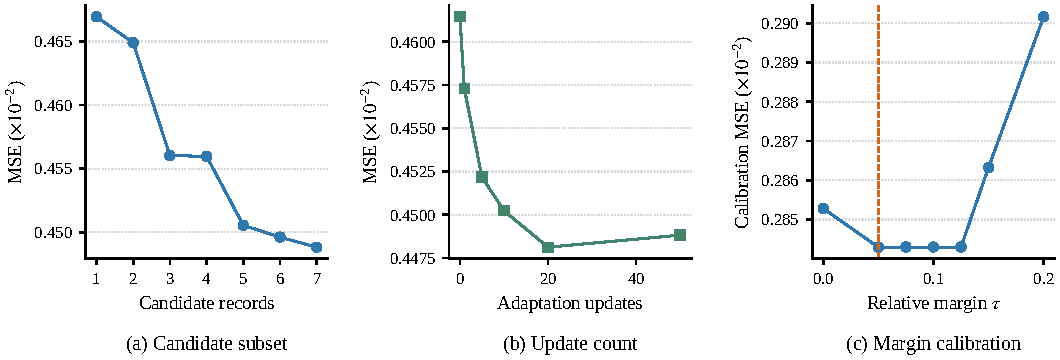
\includegraphics[width=\linewidth]{figS1.pdf}
\caption{Component sensitivities: (a) nested candidate subsets, (b) adaptation
updates with seven candidates, and (c) the primary calibration-margin curve.
Panels (a)--(b) report evaluation MSE; panel (c) reports calibration MSE.}
\label{fig:configuration}
\end{figure}

The subset curve improves from 0.004669 with A55 alone to 0.004488 with seven
records. The update curve is nonmonotonic: 20 updates yield 0.004481,
slightly below 0.004488 at 50 updates, and agree with the 50-update candidate
selection in 82.5\% of tasks. Thus, the results do not imply that additional
adaptation steps always improve selection.

\begin{table}[!htbp]
\centering\footnotesize
\begin{minipage}[t]{.43\linewidth}
\centering
\caption{Nested candidate-subset sensitivity.}\label{tab:s-bankcurve}
\begin{tabular}{rrr}
\toprule Records & $\tau$ & MSE\\\midrule
1 & 0 & 0.00466938\\
2 & 0 & 0.00464900\\
3 & 0.05 & 0.00456028\\
4 & 0.05 & 0.00455966\\
5 & 0.05 & 0.00450548\\
6 & 0.05 & 0.00449615\\
7 & 0.05 & 0.00448824\\
\bottomrule\end{tabular}
\end{minipage}\hfill
\begin{minipage}[t]{.53\linewidth}
\centering
\caption{Adaptation-update sensitivity.}\label{tab:s-updates}
\begin{tabular}{rrrr}
\toprule Updates & $\tau$ & MSE & Agreement\\\midrule
0 & 0 & 0.00461449 & 60.83\%\\
1 & 0 & 0.00457297 & 59.17\%\\
5 & 0 & 0.00452183 & 55.00\%\\
10 & 0.075 & 0.00450235 & 65.00\%\\
20 & 0.05 & 0.00448124 & 82.50\%\\
50 & 0.05 & 0.00448824 & 100.00\%\\
\bottomrule\end{tabular}
\end{minipage}
\par\vspace{4pt}\begin{minipage}{\linewidth}\footnotesize
Subsets follow the order stated in Section~S5. Each subset/update condition
has its own calibrated margin. Agreement compares candidate identities
with those selected after 50 updates.
\end{minipage}
\end{table}


The matched-optimizer comparisons in Table~\ref{tab:s-matched} use SGD/MSE,
50 updates, learning rate 0.01, and clipping at one for every adapted candidate.
The A55 shortlist combines A55 with the first 11 non-A55 configurations in
the fused-ranking shortlist, using their source-trained initializations.
The A57-PT shortlist is formed analogously. Within each shortlist, calibrated
reference-based selection and direct validation minimization share identical
candidates, adaptation, and scores. The last two controls apply the matched
optimizer to the fused-ranking and support-proxy NAS shortlists.

\begin{table}[!htbp]
\centering\footnotesize
\caption{Matched-optimizer controls (errors in $10^{-2}$ units).}\label{tab:s-matched}
\begin{tabular}{lrrrrrr}
\toprule
Selection policy & $\tau$ & MSE & MAE & Worst-10\% & CVaR90 & Harm\\\midrule
A55 shortlist, calibrated & 0.2 & 0.4472 & 1.9689 & 2.8063 & 3.6736 & 0.00\%\\
A55 shortlist, validation minimum & 0 & 0.4429 & 1.9353 & 2.7722 & 3.6736 & 0.00\%\\
A57-PT shortlist, calibrated & 0.2 & 0.4634 & 1.9798 & 2.8973 & 3.8389 & 0.00\%\\
A57-PT shortlist, validation minimum & 0 & 0.4614 & 1.9629 & 2.8837 & 3.8389 & 0.83\%\\
Fused ranking, SGD50 & 0 & 0.7790 & 2.5407 & 4.6905 & 6.4468 & --\\
Support proxy, SGD50 & 0 & 0.7306 & 2.4666 & 4.4837 & 6.0922 & --\\
\bottomrule\end{tabular}
\par\vspace{3pt}\begin{minipage}{\linewidth}\footnotesize Each calibrated policy and its validation-minimum counterpart share the same task-specific shortlist and source checkpoints. Harm is relative to the named adapted reference; the last two controls have no reference-based policy.\end{minipage}
\end{table}


Direct validation minimization improves MSE from 0.004472 to 0.004429 in the
A55 shortlist, with zero harmful selections for both policies. In the A57-PT
shortlist it improves MSE from 0.004634 to 0.004614, while harmful selections
increase from zero to one of 120 tasks. The relative-margin effect varies
with the shortlist and reference.

\section{Source and Architecture-Preselection Sensitivity}
Table~\ref{tab:s-source} reports all source-pool and source-seed conditions.
The source pools are nested; feature normalization remains fitted to the
20-VM source pool. Each trained bank receives a development-selected reference
and a calibrated margin. The seed-2905 and seed-2906 banks have evaluation
harm rates of 11.67\% and 5.83\%, exceeding the 5\% empirical calibration
criterion. Source training affects both prediction error and selection harm.

\begin{table}[pos=!htbp]
\centering\footnotesize
\caption{Source-training sensitivity (errors in $10^{-2}$ units).}\label{tab:s-source}
\begin{tabular}{llrrrrrr}
\toprule
VMs / seed & Ref. & $\tau$ & MSE & MAE & Worst-10\% & CVaR90 & Harm\\\midrule
5 / 2904 & A57-PT & 0.125 & 0.9253 & 3.1955 & 3.5559 & 7.8912 & 2.50\%\\
10 / 2904 & A57-PT & 0.075 & 0.5778 & 2.5996 & 3.2157 & 4.6889 & 3.33\%\\
15 / 2904 & A56 & 0 & 0.4658 & 2.2216 & 2.8728 & 3.7903 & 2.50\%\\
20 / 2904 & A55 & 0.05 & 0.4488 & 2.0543 & 2.8011 & 3.6825 & 4.17\%\\
20 / 2905 & A56 & 0 & 0.4728 & 2.1490 & 2.9780 & 3.8825 & 11.67\%\\
20 / 2906 & A57-PT & 0 & 0.4518 & 2.0789 & 2.8611 & 3.6657 & 5.83\%\\
\bottomrule
\end{tabular}
\par\vspace{3pt}\begin{minipage}{\linewidth}\footnotesize All rows use the same evaluation VMs and 20-VM source-fitted normalization. References and margins are selected separately for each bank; harm is relative to that bank\textquotesingle s reference.\end{minipage}
\end{table}


Table~\ref{tab:s-preselection} examines an additional bank-construction
condition using Bitbrains development cases for architecture preselection.
Three disjoint subsets contain seven, seven, and six VMs; their union is the
full 20-VM development pool. Architecture evidence counts use these subsets
or their union, after which retained configurations receive source training.
Reference designation uses Dev20 and margin calibration uses Cal20. This
diagnostic condition shares development data between architecture
preselection and reference designation. The primary bank in Section~S2 uses
the separate synthetic preselection cases.

\begin{table}[!htbp]
\centering\footnotesize
\caption{Development-pool preselection sensitivity at the medium budget.}\label{tab:s-preselection}
\begin{tabular}{lrrrrrlrrr}
\toprule
Pool & VMs & Tasks & $t=1$ & $t=2$ & $t=3$ & Ref. & $\tau$ & MSE ($10^{-2}$) & Harm\\\midrule
Full Dev & 20 & 80 & 28 & 22 & 8 & A61 & 0 & 0.4464 & 10.00\%\\
Subset 1 & 7 & 28 & 19 & 13 & 3 & A61 & 0.05 & 0.4516 & 11.67\%\\
Subset 2 & 7 & 28 & 11 & 8 & 2 & A55 & 0.05 & 0.4444 & 10.00\%\\
Subset 3 & 6 & 24 & 11 & 9 & 5 & A57-PT & 0 & 0.4575 & 5.00\%\\
\bottomrule\end{tabular}
\par\vspace{3pt}\begin{minipage}{\linewidth}\footnotesize Threshold columns count retained architecture configurations. Downstream banks use $t=2$ and include A57-PT as an additional reusable record. The three subsets partition the 20-VM development pool; the full-pool analysis overlaps all three.\end{minipage}
\end{table}


The threshold-two architecture counts range from eight to 22 across pools.
At the medium budget, MSE ranges from 0.004444 to 0.004575 and harm from
5.00\% to 11.67\%. Bank construction changes the feasible alternatives,
the selected reference, and the calibrated policy. The full-pool condition
overlaps its three subsets, so these four results are dependent sensitivity
conditions. The accompanying CSV includes tight and loose budgets as well.

\section{Resource Constraints and Measured Computation}
The primary bank has seven records at the medium and loose budgets and four
at the tight budget. Under the tight budget, all seven records satisfy the
operation limit, while the three MLP records exceed the parameter limit.
The eight-record stress bank adds the source-trained temporal convolutional
configuration A24. Its joint parameter and operation limits are 79554.5 and
1124496, respectively. Table~\ref{tab:s-constraints} compares jointly enforced
and single-active-limit conditions, each with its own calibrated margin.

\begin{table}[pos=!htbp]
\centering\footnotesize
\caption{Resource-constraint diagnostics (MSE in $10^{-2}$ units).}\label{tab:s-constraints}
\begin{tabular}{llrrrr}
\toprule
Bank & Active limits & Feasible & $\tau$ & MSE & Harm\\\midrule
Q7 (tight) & Both & 4 & 0.05 & 0.4532 & 2.50\%\\
Q7 (tight) & Operations only & 7 & 0.05 & 0.4488 & 4.17\%\\
Q7 (tight) & Parameters only & 4 & 0.05 & 0.4532 & 2.50\%\\
Q8 (stress) & Both & 6 & 0.05 & 0.4489 & 4.17\%\\
Q8 (stress) & Operations only & 7 & 0.05 & 0.4488 & 4.17\%\\
Q8 (stress) & Parameters only & 7 & 0.05 & 0.4428 & 4.17\%\\
\bottomrule
\end{tabular}
\par\vspace{3pt}\begin{minipage}{\linewidth}\footnotesize Each constraint condition has its own calibration. For the eight-record stress bank, parameter-only selection violates the operation limit in 16 tasks, and operation-only selection violates the parameter limit in two tasks.\end{minipage}
\end{table}


With the eight-record bank, operation-only selection violates the joint
parameter limit in two tasks; parameter-only selection violates the joint
operation limit in 16 tasks. Both bounds have observable effects
when they constrain different candidate records.

The hardware measurements use Windows 11, Python 3.13.5, PyTorch 2.13.0 with
CUDA 12.6, and an NVIDIA GeForce RTX 3060 Laptop GPU. Table~\ref{tab:s-latency}
reports the five executable structures at both horizons on CPU and GPU.
Each setting uses an input tensor of shape $1\times96\times25$, 100 warmup
calls, and five batches of 1000 timed calls. The CPU runs with one thread;
GPU measurements synchronize around the timed forward pass. A deterministic
zero-valued input standardizes this computation benchmark. Parameter
and operation counts describe model complexity; latency also includes
framework, device, and sequence-execution overhead.

\begin{table}[!htbp]
\centering\footnotesize
\caption{Single-window inference latency on the measured host (milliseconds).}\label{tab:s-latency}
\begin{tabular}{lrrrrrrr}
\toprule
Structure & $H$ & Params. & Ops. & CPU median & CPU p95 & GPU median & GPU p95\\\midrule
A1 & 1 & 77921 & 155712 & 0.0451 & 0.0533 & 0.1469 & 0.2065\\
A1 & 4 & 78020 & 155904 & 0.0452 & 0.0558 & 0.1322 & 0.2621\\
A6 & 1 & 78977 & 157760 & 0.0463 & 0.0551 & 0.1627 & 0.3414\\
A6 & 4 & 79076 & 157952 & 0.0462 & 0.0768 & 0.1485 & 0.2365\\
A13 & 1 & 80033 & 159808 & 0.0732 & 0.1105 & 0.2207 & 0.4686\\
A13 & 4 & 80132 & 160000 & 0.0731 & 0.0857 & 0.2025 & 0.2779\\
A55 & 1 & 2081 & 377888 & 1.9381 & 2.3867 & 5.9565 & 8.0760\\
A55 & 4 & 2132 & 377984 & 1.9492 & 2.4966 & 5.8619 & 7.2274\\
A56/A57 & 1 & 5697 & 1050688 & 1.9588 & 2.3125 & 5.9442 & 10.0755\\
A56/A57 & 4 & 5796 & 1050880 & 1.9688 & 2.4392 & 5.8404 & 7.2944\\
\bottomrule\end{tabular}
\par\vspace{3pt}\begin{minipage}{\linewidth}\footnotesize Each device/structure/horizon setting includes 100 warmup calls and 5000 timed calls. CPU inference uses one thread; GPU calls are synchronized. Latencies include framework and device overhead.\end{minipage}
\end{table}


Target-pipeline timing uses calibration VM 1204, four horizon/support
conditions, and three deployment budgets. Each method/condition has one
warmup and five measured repetitions. The timed region includes checkpoint
loading, model construction, search proxies where applicable, adaptation,
validation, feasibility masking, and selection. Offline source training,
prefix construction, and subsequent forecast evaluation are separate stages.
The MSA-DTI implementation executes all seven candidate adaptations before
budget masking, giving mean runtime 8.124~s versus 1.971~s for PT+FT.
These measurements describe seven-candidate execution. The feasibility-first
algorithm in the main article instead scales its adaptation work with the
feasible subset. The file \texttt{pipeline\_timing.csv} supplies the 96
method/condition summaries for the eight methods, including repetition
counts, means, standard deviations, and ranges.

\section{Accompanying Data and Figure Reproduction}
The LaTeX project includes plot-ready data and the manuscript figures.
The data directory contains per-task errors, candidate identities, resource
counts, and control results. The Python scripts reproduce experimental Figures
5--9 from the accompanying plot-ready data. The selection-rule code and
manuscript sources are available in Release v1.3.4 at
\url{https://github.com/w924871681/paper-code-DT-Twin/releases/tag/v1.3.4}.
The accompanying numerical records reproduce the reported summary statistics.
Raw workload traces are obtained from the Grid Workloads Archive at
\url{https://atlarge-research.com/gwa-t-12/}.

\end{document}

